\subsection{Simplicial complexes}

A \emph{simplicial complex} may be considered as an embedding of points, line segments, triangles, and $n$-dimensional counterparts in Euclidean space; however, it is often beneficial to look at simplicial complexes as a purely combinatorial object; we omit details on how it will be embedded into Euclidean space. Strictly, this combinatorial view would be referred to as an \emph{abstract simplicial complex}, but we will refer to it as a \emph{simplicial complex}.

\begin{definition}[Simplicial complex]
    An \emph{simplicial complex} is a family of sets that is closed under taking subsets.
\end{definition}

Note the existence of the empty simplex that arises from this definition. Some definitions chose to disregard this as a valid simplex, and we will do so here.

\begin{definition}
    Let $K$ be a simplicial complex.
    \begin{enumerate}
        \item An element $\sigma \in K$ is called a \emph{$p$-simplex}, where $p = \dim\sigma = \lvert \sigma \rvert - 1$.
        \item Let $\sigma$ be a $p$-simplex. An element $\tau \subset \sigma$ is called a \emph{face} of $\sigma$.
        \item Let $\sigma$ be a $p$-simplex. An element $\tau \supset \sigma$ is called a \emph{coface} of $\sigma$.
        \item Let $\tau$ be a face of a $p$-simplex $\sigma$, where $p \geq 0$. If $\dim\tau = p-1$, then $\tau$ is called a facet of $\sigma$.
        \item Let $\tau$ be a coface of a $p$-simplex $\sigma$. If $\dim\tau = p+1$, then $\tau$ is called a cofacet of $\sigma$.
        \item $\restr Kp$ denotes the set of $p$-simplices in $K$ (this is not typically a simplicial complex).
        \item The \emph{$p$-skeleton} of $K$ is defined as $\sk_p(K) = \bigcup_{i \in \{0, \ldots, p\}} \restr Ki$.
        \item The dimension of $K$ is the greatest $p$ such that $\restr Kp$ is non-empty, denoted by $\dim K$.
        \item A simplicial complex $K'$ is said to be a \emph{subcomplex} of $K$ if $K' \subset K$.
        \item $K$ is said to be finite if $\lvert K \rvert < \infty$.
    \end{enumerate}
\end{definition}
We will be working exclusively with finite simplicial complex, so we assume all simplicial complexes are finite unless otherwise stated.

An \emph{orientation} of a $k$-simplex $\sigma = \{v_0, \ldots, v_k\}$ is an equivalence class of the orderings of the vertices of $\sigma$. We let $(v_0, \ldots, v_k) \sim (v_{\tau(0)}, \ldots, v_{\tau(k)})$ if the sign of the permutation $\tau$ is $1$. Denote an oriented simplex by $[\sigma]$, and denote the set of oriented $p$-simplices of $K$ by $\left[\restr Kp\right]$.

\begin{figure}
    \centering
    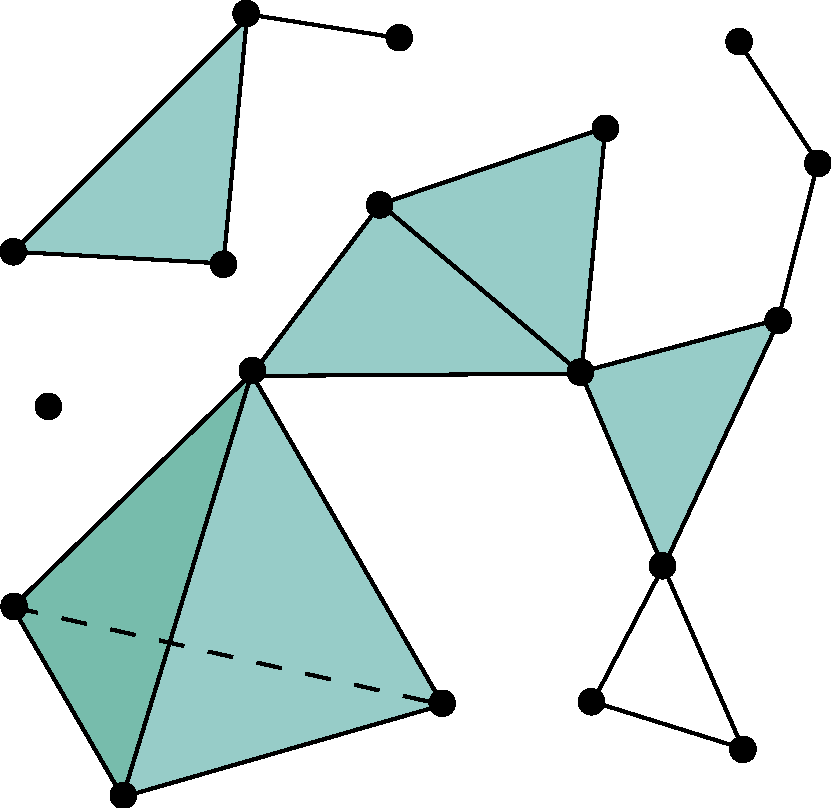
\includegraphics[width=0.6\textwidth]{content/2-background/images/simplicial-complex}
    \caption{A simplicial complex of dimension $3$.}
    \label{fig:simplicial-complex}
\end{figure}

Although we ignore the details of embedding, it is often useful to visualise simplicial complexes in $\mathbb R^2$, see Figure \ref{fig:simplicial-complex}.

\begin{definition}[Simplicial chain complex]
    \label{def:simplicial-chain-complex}
    Let $K$ be a simplicial complex and $R$ be a commutative ring. The \emph{simplicial chain complex of $K$ with coefficients in $R$} is a chain complex $C(K; R) = (C_*, \partial_*)$ where
    \begin{align*}
        C_i                            & = R \left\langle \left[\restr{K}{i}\right] \right\rangle           \\
        \partial_i([v_0, \ldots, v_i]) & = \sum_{j=0}^i (-1)^j [v_0, \ldots, v_{j-1}, v_{j+1}, \ldots, v_i]
    \end{align*}
    where $[v_0, \ldots, v_i]$ is an oriented $i$-simplex. We extend $\partial_i$ to the full domain of $C_i$ by extending linearly.
\end{definition}

\begin{example}
    We consider the simplicial complex $K$ consisting of the $2$-simplex $[a,b,c]$ and all of its faces. Let $(C_*, \partial_*) = C(K; \mathbb Z)$. We will present the boundary maps as matrices, so we pick the basis $([a],[b],[c])$ for $C_0$, $([ab], [ac], [bc])$ for $C_1$, and $([abc])$ for $C_2$. Thus we have
    \begin{align*}
        C_0 & \cong \mathbb Z^3, & M_{\partial_0} & =
        \begin{blockarray}{cccc}
            & [a] & [b] & [c] \\
            \begin{block}{c(ccc)}
                {[0]} & 0 & 0 & 0 \\
            \end{block}
        \end{blockarray} ;                      \\
        C_1 & \cong \mathbb Z^3, & M_{\partial_1} & =
        \begin{blockarray}{cccc}
            & [ab] & [ac] & [bc] \\
            \begin{block}{c(ccc)}
                {[a]} & -1 & -1 & 0 \\
                {[b]} & 1 & 0 & -1 \\
                {[c]} & 0 & 1 & 1 \\
            \end{block}
        \end{blockarray}\;;                      \\
        C_2 & \cong \mathbb Z,   & M_{\partial_2} & =
        \begin{blockarray}{cc}
            & [abc] \\
            \begin{block}{c(c)}
                {[ab]} & 1 \\
                {[ac]} & -1 \\
                {[bc]} & 1 \\
            \end{block}
        \end{blockarray}\;.
    \end{align*}
\end{example}

\begin{definition}[Simplicial homology]
    Let $K$ be a simplicial complex and $R$ be a commutative ring. Then the \emph{$n$th homology group} of $K$ is defined as the homology of the simplicial chain complex of $K$; that is,
    \[ H_n(K; R) = H_n(C(K; R)). \]
    When $R = \mathbb Z$, we simply write $H_n(K; \mathbb Z) = H_n(K)$.
\end{definition}

\begin{example}
    We now present some worked examples of homology on simplicial complexes. Note here we are using a shorthand, so $a$ strictly should be written $\{a\}$ and $ab$ similarly should be written $\{a, b\}$.
    \begin{enumerate}
        \item Let $K$ be the simplicial complex with $0$-simplices $[a_1], \ldots, [a_n]$ and a $1$-simplex $[a_i,a_{i+1}]$ for each $i \in \{1, \ldots, n-1\}$. We consider the chain complex of $K$, $C(K;\mathbb Z) = (C_*, \partial_*)$:
              \[ 0 \to \mathbb Z^{n-1} \xrightarrow{\partial_1} \mathbb Z^n \to 0. \]
              For $C_0$ we pick the basis $([a_1], \ldots, [a_n])$, and for $C_1$ we pick the basis $([a_1a_2], \ldots, [a_{n-1}a_n])$. Firstly, as $C_i = 0$ for all $i \geq 2$, $H_i(K) = 0$ for all $i \geq 2$. We now look at the matrix representation of $\partial_1$.
              \[
                  \begin{blockarray}{ccccccc}
                      & [a_1a_2] & [a_2a_3] & [a_3a_4] & \ldots & [a_{n-2}a_{n-1}] & [a_{n-1}a_n] \\
                      \begin{block}{c(cccccc)}
                          {[a_1]} & -1     & 0      & 0      & \ldots & 0      & 0      \\
                          {[a_2]} & 1      & -1     & 0      & \ldots & 0      & 0      \\
                          {[a_3]} & 0      & 1      & -1     & \ldots & 0      & 0      \\
                          {[a_4]} & 0      & 0      & 1      & \ldots & 0      & 0      \\
                          \ldots & \vdots & \vdots & \vdots & \ddots & \vdots & \vdots \\
                          {[a_{n-1}]} & 0      & 0      & 0      & \ldots & 1      & -1     \\
                          {[a_n]} & 0      & 0      & 0      & \ldots & 0      & 1      \\
                      \end{block}
                  \end{blockarray}
              \]
              By performing the row operations $R_i \gets R_i + R_{i-1}$ in the order $i \in \{2, 3, \ldots, n\}$, we get the following matrix (that is in Smith normal form).
              \[
                  \begin{pmatrix}
                      -1     & 0      & 0      & \ldots & 0      & 0      \\
                      0      & -1     & 0      & \ldots & 0      & 0      \\
                      0      & 0      & -1     & \ldots & 0      & 0      \\
                      0      & 0      & 0      & \ldots & 0      & 0      \\
                      \vdots & \vdots & \vdots & \ddots & \vdots & \vdots \\
                      0      & 0      & 0      & \ldots & 0      & -1     \\
                      0      & 0      & 0      & \ldots & 0      & 0      \\
                  \end{pmatrix}
              \]
              Thus we read off the kernel and image of $\partial_1$:
              \[ \im\partial_1 = \mathbb Z^{n-1}, \qquad \ker\partial_1 = 0. \]
              Thus we get
              \[ H_0(K) = \frac{\mathbb Z^n}{\im\partial_1} = \mathbb Z, \qquad
                  H_1(K) = \frac{0}{0} = 0. \]
              The $0$th and $1$st integral homology groups of graphs have quite succinct interpretations: the rank of the $0$th homology group corresponds to the number of connected components there are and the rank of the $1$st homology group corresponds to the number of \emph{linearly independent cycles} there are. In this example, we have the path graph, which has one connected component and no cycles.

        \item We let $K$ be the simplicial complex with two $0$-simplices, $[a]$ and $[b]$, and $n$ $1$-simplices of the form $[a,b]$. We have the chain complex $(C_*, \partial_*) = C(K; \mathbb Z)$ written as
              \[ 0 \to \mathbb Z^n \xrightarrow{\partial_1} \mathbb Z^2 \to 0. \]
              Again we have $C_i = 0$ for $i \geq 2$, thus $H_i(K) = 0$ for $i \geq 2$. We have the following matrix representation of $\partial_1$.
              \[
                  \begin{blockarray}{cccccc}
                      & [ab] & [ab] & [ab] & \ldots & [ab] \\
                      \begin{block}{c(ccccc)}
                          {[a]} & -1 & -1 & -1 & \ldots & -1 \\
                          {[b]} & 1  & 1  & 1  & \ldots & 1\\
                      \end{block}
                  \end{blockarray}
              \]
              This reduces to the following matrix.
              \[
                  \begin{pmatrix}
                      1 & 0 & 0 & \ldots & 0 \\
                      0 & 0 & 0 & \ldots & 0 \\
                  \end{pmatrix}
              \]
              Thus we get
              \[ \im\partial_1 = \mathbb Z, \qquad \ker\partial_1 = \mathbb Z^{n-1}. \]
              Therefore,
              \[ H_0(K) = \mathbb Z^2 / \mathbb Z = \mathbb Z, \qquad
                  H_1(K) = \mathbb Z^{n-1} / 0 = \mathbb Z^{n-1}. \]
              To interpret this example, we have two points and $n$ edge connecting them; thus, we have $1$ connected component and $n-1$ linearly independent cycles.
        \item Our last example moves away from graphs. Consider the simplicial complex $K$ consisting of all proper faces of the $3$-simplex $[a,b,c,d]$.
              We may think of $K$ as a the boundary of a tetrahedron (homeomorphic to $S^2$). We have the following integral chain complex.
              \[ 0 \to \mathbb Z^4 \xrightarrow{\partial_2} \mathbb Z^6 \xrightarrow{\partial_1} \mathbb Z^4 \to 0. \]
              We now look the matrix representations of the (non-trivial) boundary maps and their reduction.
                  {\small
                      \begin{align*}
                          M_{\partial_1} & =
                          \begin{blockarray}{ccccccc}
                              & [ab] & [ac] & [ad] & [bc] & [bd] & [cd] \\
                              \begin{block}{c(cccccc)}
                                  {[a]} & -1 & -1 & -1 & 0  & 0  & 0  \\
                                  {[b]} & 1  & 0  & 0  & -1 & -1 & 0  \\
                                  {[c]} & 0  & 1  & 0  & 1  & 0  & -1 \\
                                  {[d]} & 0  & 0  & 1  & 0  & 1  & 1  \\
                              \end{block}
                          \end{blockarray}
                          \to
                          \begin{pmatrix}
                              1 & 0 & 0 & 0 & 0 & 0 \\
                              0 & 1 & 0 & 0 & 0 & 0 \\
                              0 & 0 & 1 & 0 & 0 & 0 \\
                              0 & 0 & 0 & 0 & 0 & 0 \\
                          \end{pmatrix} \\
                          M_{\partial_2} & =
                          \begin{blockarray}{ccccc}
                              & [abc] & [abd] & [acd] & [bcd] \\
                              \begin{block}{c(cccc)}
                                  {[ab]} & 1  & 1  & 0  & 0  \\
                                  {[ac]} & -1 & 0  & 1  & 0  \\
                                  {[ad]} & 0  & -1 & -1 & 0  \\
                                  {[bc]} & 1  & 0  & 0  & 1  \\
                                  {[bd]} & 0  & 1  & 0  & -1 \\
                                  {[cd]} & 0  & 0  & 1  & 1  \\
                              \end{block}
                          \end{blockarray}
                          \to
                          \begin{pmatrix}
                              1 & 0 & 0 & 0 \\
                              0 & 1 & 0 & 0 \\
                              0 & 0 & 1 & 0 \\
                              0 & 0 & 0 & 0 \\
                              0 & 0 & 0 & 0 \\
                              0 & 0 & 0 & 0 \\
                          \end{pmatrix}        \\
                          M_{\partial_3} & =
                          \begin{blockarray}{cc}
                              & [abcd] \\
                              \begin{block}{c(c)}
                                  {[abc]} & -1 \\
                                  {[abd]} & 1  \\
                                  {[acd]} & -1 \\
                                  {[bcd]} & 1  \\
                              \end{block}
                          \end{blockarray}
                          \to
                          \begin{pmatrix}
                              1 \\ 0 \\ 0 \\ 0
                          \end{pmatrix}
                      \end{align*}
                  }
              Thus we get the homology groups
              \[
                  H_n(K) = \begin{cases}
                      \mathbb Z & n \in \{0, 2\},   \\
                      0         & \text{otherwise}.
                  \end{cases}
              \]
              The rank of the $0$th homology group can still be interpreted as the number of connected component. The rank of the $2$th homology group can be interpreted as the number of $2$-dimensional \emph{holes} in $K$ (or $S^2$); that is, the number of \emph{voids}. As our tetrahedron is hollow, it has one void (precisely the space the boundary encompasses)
    \end{enumerate}
\end{example}

\emph{Filtrations} are widely used in algebraic topology (particularly in homological algebra). We have already seen gradings for rings (and modules), and these two are closely linked. 

\begin{definition}[Filtration]
    A \emph{filtration} is a family $\{S_i\}_{i \in \mathcal I}$ of subobjects of a given structure $S$, where $\mathcal I$ is some totally ordered set, and for $i, j \in I$ we have
    \[ i \leq j \implies S_i \subset S_j. \]
\end{definition}

A filtered ring is a generalisation of a graded ring. 

\begin{definition}[Filtered simplicial complex]
    A \emph{filtered simplicial complex} is a filtration of simplicial complexes $\mathbb K = \{K_i\}_{i \in \mathcal I}$ (that is, if $i < j$, then $K_i$ is a subcomplex of $K_j$). 
\end{definition}

We will be working with finite filtered simplicial complexes. Thus, as with our definition of grading, we will take $\mathcal I = \{0, \ldots, n\}$ for some $n \in \N$. A filtration of a simplicial complex $K$ is a filtered simplicial complex $\mathbb K = (K_i)_{i=0}^n$ such that $K_n = K$. 

\begin{figure}[b]
    \centering
    \begin{subfigure}[t]{0.49\textwidth}
        \centering
        \fbox{
            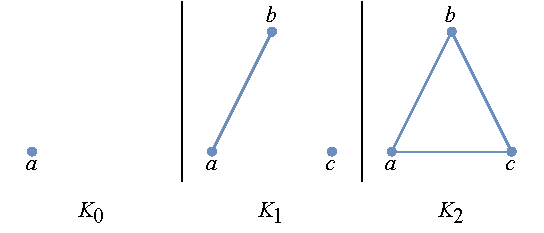
\includegraphics[width=0.9\textwidth]{content/2-background/images/filtration-ex-1.pdf}
        }
        \caption{A valid filtered simplicial complex, each filtration level is a subset of the next and are all valid simplicial complexes.}
        \label{fig:filtration-ex-1}
    \end{subfigure}
    \begin{subfigure}[t]{0.49\textwidth}
        \centering
        \fbox{
            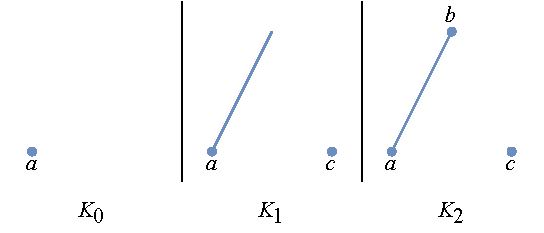
\includegraphics[width=0.9\textwidth]{content/2-background/images/filtration-ex-2.pdf}
        }
        \caption{An invalid filtered simplicial complex, each filtration level is a subset of the next, but $K_1$ is not a valid simplicial complex.}
        \label{fig:filtration-ex-2}
    \end{subfigure}
    \caption{Two sequences of simplicial complex, one that defines a filtration and another that does not.}
\end{figure}

\begin{example}
    We consider two examples, one that is a valid filtered simplicial complex and another that is not. 
    \begin{enumerate}
        \item Consider the sequence
              \[ \underbrace{\{a\}}_{K_0} \subset \underbrace{\{a, b, c, ab\}}_{K_1} \subset \underbrace{\{a, b, c, ab, ac, bc\}}_{K_2}. \]
              This is indeed a filtered simplicial complex, as shown in Figure \ref{fig:filtration-ex-1}.
        \item Consider the sequence
              \[ \underbrace{\{a\}}_{K_0} \subset \underbrace{\{a, c, ab\}}_{K_1} \subset \underbrace{\{a, b, c, ab\}}_{K_2}. \]
              This is \emph{not} a filtered complex, although each level is a subset of the next, observe that $ab \in K_1$ but $ab \supset b \not\in K_1$.
    \end{enumerate}
\end{example}

We note that a maximal filtration of simplicial complexes induces an ordering on the simplices. For example, consider the filtered simplicial complex
\[\{\{1\}\} \subset \{\{1\}, \{2\}\} \subset \{\{1\}, \{2\}, \{1,2\}\}.\]
This filtration corresponds to the ordering $(\{1\}, \{2\}, \{1,2\})$.

For a non-maximal filtration of simplicial complexes, there are multiple induced orderings. For example, consider the filtered simplicial complex
\[\{\{1\}, \{2\}\} \subset \{\{1\}, \{2\}, \{1,2\}\}.\]
This may correspond to the ordering above or $(\{2\}, \{1\}, \{1,2\})$. We call such a corresponding ordering a \emph{compatible ordering of simplices} from the filtration.

% We now reintroduce persistence with a simplified view, then connect it to the structure we previously established.

% \begin{definition}[Persistent homology]
%     Let $\mathbb K = (K_i)_{i=0}^n$ be a finite filtered simplicial complex, $\mathbb F$ be a field, and let $(C^i_*, \partial^i_*) = C(K_i; \mathbb F)$. Fix $i \in \mathbb N_0$. We define the $p$-persistent $n$th homology group of $K_i$ as
%     \[ H^{i,p}_n(\mathbb K) = \frac{\ker\partial^i_n}{\im\partial_{n+1}^{i+p} \cap \ker\partial_n^i}. \]
% \end{definition}

\begin{lemma}
    Any filtered simplicial complex is a persistence complex.
\end{lemma}

\begin{proof}
    As in Definition \ref{def:simplicial-chain-complex}, we take $C^i = C(K_i; R) = (C^i_*, \partial^i_*)$ for some commutative ring $R$. For the chain maps, we use the inclusion map: $f^i = \iota_i: C^i_* \to C^{i+1}_*$. It is clear that these are in fact chain maps.
\end{proof}

\begin{definition}[Persistence barcodes of a filtered simplicial complex]
    Let $\mathbb K = \{K_i\}_{i=0}^n$ be a filtered simplicial complex. The \emph{persistence barcodes} of $H_*(\mathbb K)$ are simply the persistence barcodes of the homology of the corresponding persistence complex $\mathcal C$; that is,
    \[ \Pers(H_*(\mathbb K)) = \Pers(H_*(\mathcal C)). \]
\end{definition}

\begin{figure}
    \centering
    \begin{subfigure}[b]{0.95\textwidth}
        \centering
        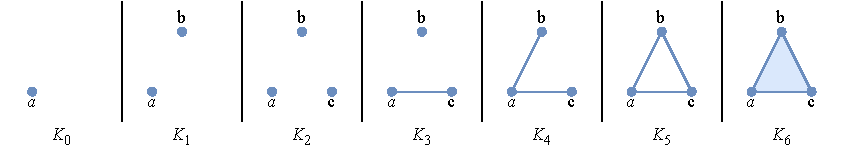
\includegraphics[width=\textwidth]{content/2-background/images/barcodes-ex-1}
        \caption{A filtered simplicial complex.}
        \label{fig:barcodes-ex-fil}
    \end{subfigure}
    \begin{subfigure}[b]{0.95\textwidth}
        \centering
        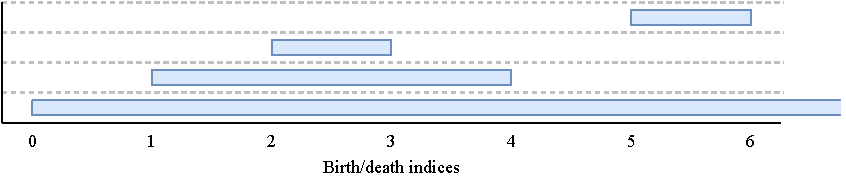
\includegraphics[width=\textwidth]{content/2-background/images/barcodes-ex-2}
        \caption{The persistent barcodes for the filtered simplicial complex. Note the barcode at the bottom corresponds to the $\mathcal P$-interval $(0, \infty)$.}
        \label{fig:barcodes-ex-barcodes}
    \end{subfigure}
    \caption{A filtered simplicial complex alongside the persistent barcode.}
    \label{fig:barcodes-ex}
\end{figure}

\begin{example}
    We consider the maximal filtered simplicial complex $\mathbb K$ corresponding to the following simplex ordering:
    \[ (a, b, c, ac, ab, bc, abc) \]
    (note we are using the shorthand $a = \{a\}$, $ab = \{a,b\}$, etc.). We detail the span of the homology classes:
    \begin{enumerate}
        \item the $0$-dimensional homology class created by $a$ persists through to the end complex;
        \item the $0$-dimensional homology class created by $b$ is killed by $ab$;
        \item the $0$-dimensional homology class created by $c$ is killed by $ac$; and
        \item the $1$-dimensional homology class created by $bc$ is killed by $abc$.
    \end{enumerate}
    Figure \ref{fig:barcodes-ex} visualises this example: in Figure \ref{fig:barcodes-ex-fil} we have a visualisation of the filtration levels of $\mathbb K$ and in Figure \ref{fig:barcodes-ex-barcodes} we have the persistent barcodes for $\mathbb K$.
\end{example}

% \begin{lemma}
%     Let $\mathbb F$ be a field, $\mathbb K = (K_i)_{i=0}^n$ be a finite filtered simplicial complex, and $\mathcal P$ be the set of $\mathcal P$-intervals of the persistence module corresponding to the persistence complex of $\mathbb K$. Let $\tau$ be the set of triangles defined by the $\mathcal P$-intervals in $\mathcal P$: for each $(i, j) \in \mathcal P$, the corresponding triangle has endpoints: $(i, 0)$, $(j, 0)$, and $(i, j - i)$. Then $\rank H^{i,p}_k(\mathbb K)$ is equal to the number of triangles in $\tau$ containing the point $(i, p)$. 
% \end{lemma}

% \begin{proof}
%     Consider a $\mathcal P$-interval $(i, j)$. This corresponds to a $n$-cycle $e$ starting at $i$ until time $j-1$. We now ask when $[e]$ is a basis element for $H^{l,p}_n(\mathbb K)$. From the definition of persistent homology, $e \not\in \im_{k+1}^l$ for $l < j$. Thus $e \not\in \im_{k+1}^{l+p}$ for $l + p < j$. We also have $l \geq i$ and $p \geq 0$, thus we have formed our triangular region.  
% \end{proof}

% We now move to interpret the work we have done on persistence modules to finite filtered simplicial complex. Let $\mathbb K = (K_i)_{i=0}^n$ be a finite filtered simplicial complex. We have seen that $\mathbb K$ becomes a persistence complex (over some field $\mathbb F$) with inclusion maps for the simplices, as shown below.
% \[ C(K_0; \mathbb F) \xhookrightarrow{\iota_0} C(K_1; \mathbb F) \xhookrightarrow{\iota_1} C(K_2; \mathbb F) \xhookrightarrow{\iota_2} \ldots \]
% By Lemma \ref{lem:persistence-complex-is-persistence-module}, we see that the homology of $\mathbb K$ forms a persistence module $H_*(\mathbb K; \mathbb F)$. In fact, as we are considering finite simplicial complexes, $\mathbb K$ is a finite type persistence complex and thus $H_*(\mathbb K; \mathbb F)$ is a finite type persistence module. Therefore, we may assign a multiset of $\mathcal P$-intervals to the $H_*(\mathbb K; \mathbb F)$. In particular, a $\mathcal P$-interval $(i, j)$ describes a basis element for the homology vector spaces which exists between $i$ and $j-1$ in the grading. We interpret this as a homology class that is \emph{born} at time $i$ and \emph{dies} at time $j$. The $\mathcal P$-intervals of the form $(i, \infty)$ are precisely the homology classes that are born at $i$ and persist through to the final complex $K_n$. 
